

% \layout
%     \setlength{\hoffset}{0pt}
%     \setlength{\voffset}{0pt}
%     \setlength{\topmargin}{0pt}
%     \setlength{\oddsidemargin}{0pt}
%     \setlength{\marginparwidth}{0pt}
%     \setlength{\marginparsep}{0pt}
%     \setlength{\textwidth}{465pt}
%     \setlength{\textheight}{600pt}
% \layout*

\section{\huge \textbf{Supporting Information}}

\beginsupplement

\subsection{Conceptualization}

\begin{figure*}[h]
    \centering
    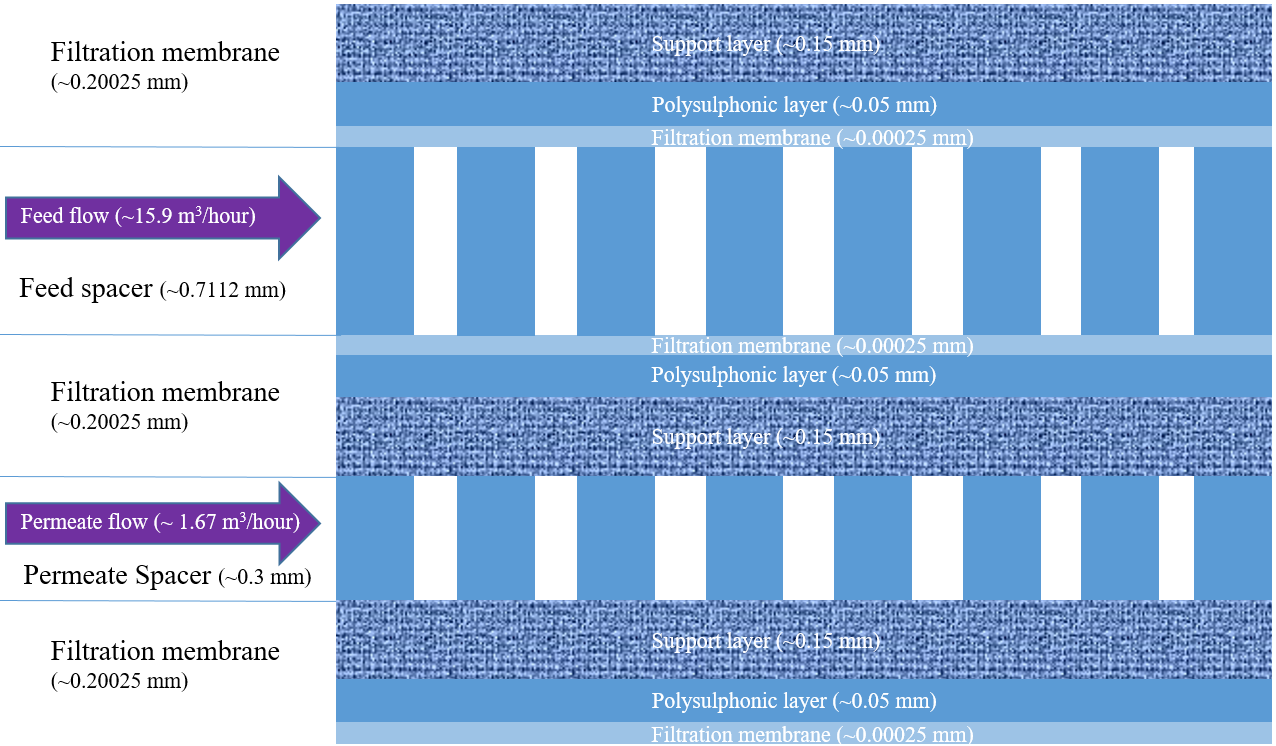
\includegraphics[width = \textwidth]{images/ROSSpy/supporting_information/membrane_scheme_3.PNG}
    \caption{
        A cross-section of the RO filtration membrane. The listed membrane dimensions and flow rates are cited in Table S1. The polyamide membrane is further detailed in literature \cite{Strubbe2018CalibrationFull-Scale}. 
    }
    \label{membrane_scheme}
\end{figure*}

\begin{figure*}[h]
    \centering
    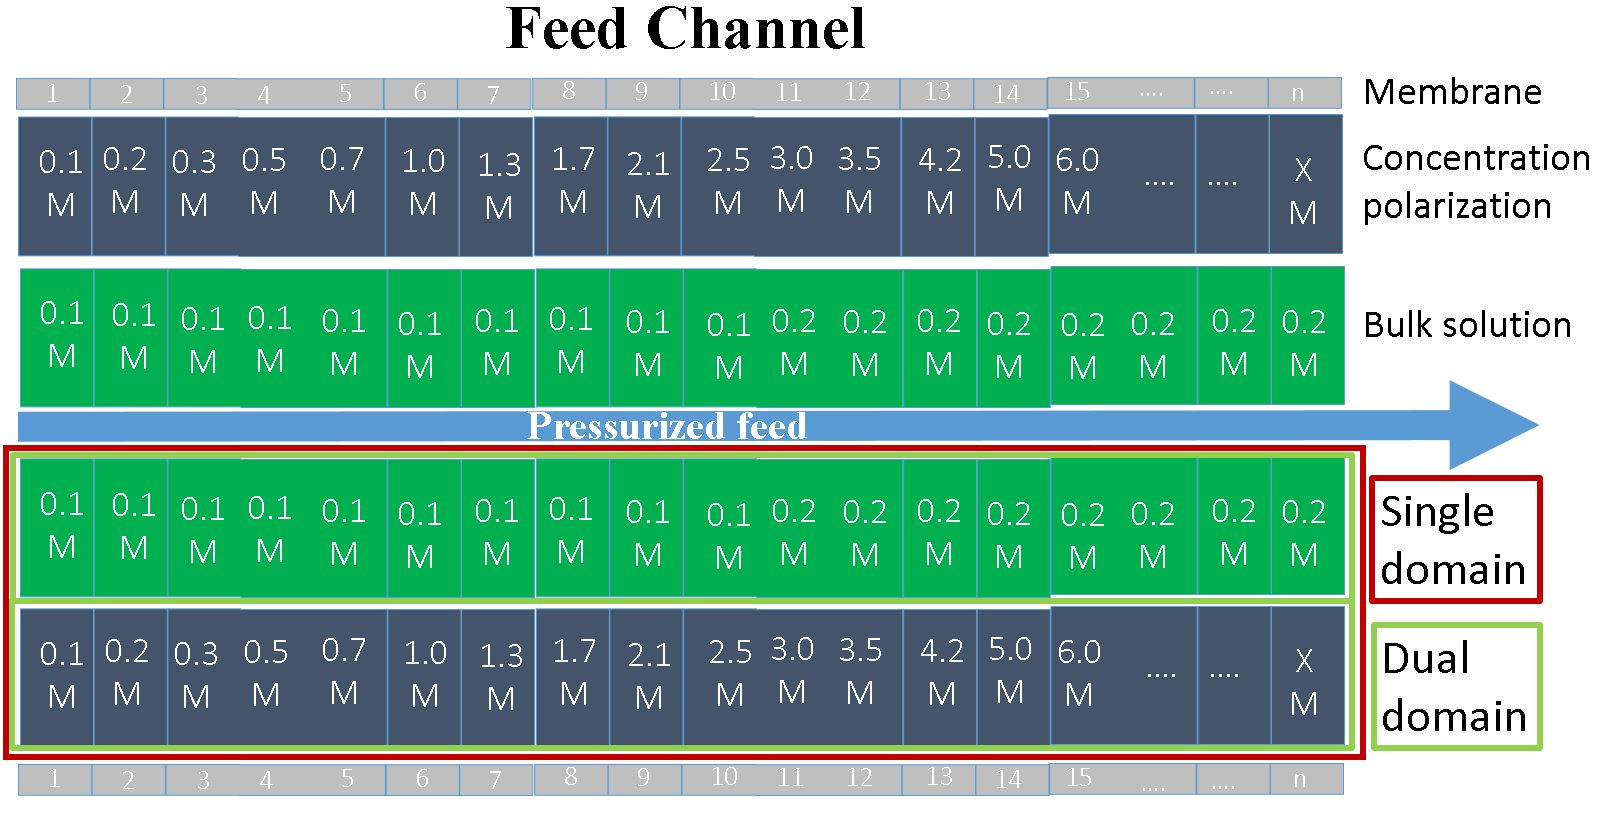
\includegraphics[width = \textwidth]{images/ROSSpy/supporting_information/single_dual_domain.jpg}
    \caption{
        A conceptual cross-section of the RO module. The membrane layers on top and bottom of the figure are discretized into an arbitrary $n$ cells. The figure illustrates the reactive transport phenomena, where the feed solution progressively becomes more concentrated as it transports through the module. The CP layer becomes much more concentrated than the bulk solution as a consequence of the no-slip boundary condition, which is granulated into a single solution by the single-domain model  yet is resolved into two distinct solutions by the dual-domain model. The boundaries of these two solution models are depicted as the red and green boxed regions, respectively. 
    }
    \label{single_dual_domain}
\end{figure*}

Cross-sections of an RO model and of the feed-membrane interface are detailed in Figures \ref{membrane_scheme}-\ref{single_dual_domain}. Figure \ref{membrane_scheme} illustrates the repeating unit of an RO filtration membrane. Figure \ref{single_dual_domain} depicts numerical reactive transport and the boundaries of the single- and dual-domain solution models.

\subsection{Software}

\begin{longtable}{c|c|c}
    \caption{
        Glossary of ROSSpy variables.  
        \label{glossary} 
    } \\ \toprule
    
    \textbf{variable} & \textbf{name} & \textbf{description} \\ \toprule
    \endfirsthead
    \multicolumn{3}{c}{continuation of Table \ref{glossary}} \\  \toprule
    \textbf{variable} & \textbf{name} & \textbf{description} \\ \toprule
    \endhead
    
    \multirow{2}{1.5em}{$l$} & \multirow{2}{3em}{length} & longitudinal dimension of the\\& & module or module cell \\ \midrule
    \multirow{2}{1.5em}{$n$} & number of & quantity of discretizations of the module \\ & module cells & \\ \midrule
    \multirow{2}{1.5em}{$\Phi$} & \multirow{2}{3em}{permeate flux} & the removed $moles_{H_2O}$ that \\& & simulates permeate flux \\ \midrule  
    $HL$ & head loss & reduction of pressure over the module distance \\ \midrule
    \multirow{2}{2em}{$PE$} & \multirow{2}{3em}{permeate efficiecy} & attenuation of permeate flux \\& & from pre-existing inefficiencies \\ \midrule  
    \multirow{2}{2em}{$CF$} & \multirow{2}{3em}{concentration factor} & solution concentration normalized \\& & to the influent concentration \\ \midrule
    $X$ & mass & water mass in the maximally filled feed channel \\ \midrule
    $V$ & velocity & feed velocity through the feed channel \\ \midrule
    $A$ & area & cross-sectional area of the RO module \\ \midrule
    $th$ & thickness & thickness of a module dimension \\ \midrule
    $Q$ & volumetric flow & feed flow through a maximally filled feed channel \\ \midrule
    \multirow{2}{1.5em}{$\Delta t$} & \multirow{2}{3em}{time} & timestep of the simulation that \\& & adheres to the Courant condition \\ \midrule
    \multirow{2}{2em}{$C_{max}$} & \multirow{2}{3em}{Courant constant} & maximal value of the Courant constant \\& & to meet the Courant condition \\ \midrule
    $\phi$ & total concentration & total ionic concentrations in the simulation \\ \midrule
    $C$ & specie concentration & concentration of an individual specie \\ \midrule
    \multirow{2}{1em}{$v$} & \multirow{2}{3em}{stoichiometry coefficient} & coefficient for the respective compound \\& & in the balanced equilibrium reaction \\ \midrule
    \multirow{2}{1em}{$N$} & number of & quantity of reactions that \\& reactions & contain a respective compound \\ \midrule
    $R$ & reaction flux & $\frac{mmol}{hour}$ flux of an equilibrium reaction \\ \midrule
    \multirow{2}{1em}{$\Omega$} & thermodynamic & logarithm of the $\frac{Q_{dissolution}}{K_{sp}}$ \\& displacement & \\ \midrule
    $k_m$ & rate constant & dissolution and precipitation rate constant \\ \midrule
    $a$ & activity & activity of the respective compound \\ \midrule
    $\eta$ & parameter & experimentally determined parameter \\ \midrule
    $p$ & parameter & experimentally determined parameter \\ \midrule
    \multirow{2}{2em}{$\Delta G$} & \multirow{2}{5em}{Gibbs free energy} & Gibbs free energy of the dissolution \\& & and precipitation reactions \\ \midrule
    $K$ & equilibrium constant & thermodynamic equilibrium of the respective reaction \\ \midrule
    $M$ & number of minerals & quantity of minerals in the studied system \\ \midrule
    $\gamma$ & activity coefficient & coefficient of metabolite activity in a respective system \\ \midrule
    $z$ & charge & compound charge of the respective metabolite \\ \midrule
    $\mu$ & ionic strength & charge-weighted concentration of a solution \\ \midrule
    $A$ & parameter & experimentally determined parameter \\ \midrule
    $B$ & parameter & experimentally determined parameter \\ \midrule
    $a_j$ & fitted parameter & parameter that is tailored to justify the system \\ \midrule
    $b_j$ & fitted parameter & parameter that is tailored to justify the system \\ \midrule
    $W_{aq}$ & water mass & mass of water in the system \\ \bottomrule
\end{longtable} 

\subsection{PHREEQC consistency}

\subsubsection{ICE table calculations}
The calculations that solve for $x$ in the presented ICE table of Table 1a. The activity coefficients ($\gamma$) for $Ca^{2+}$ and $SO_4^{2-}$ were sourced from PHREEQC for this specific solution system.
\begin{equation} \label{ice_calculations}
    \begin{split}
        K_{sp} &= [a_{Ca^{2+}} - x]^1 * [a_{SO_4^{2-}} - x]^1 \\ 
        K_{sp} &= (\gamma*[Ca^{2+}] - x) * (\gamma*[SO_4^{2-}] - x) \\ 
        10^{-4.58} &= ((0.19*0.020594) - x) * ((0.06*0.105462) - x) \\ 
        10^{-4.58} &= (0.003913 - x) * (0.00633 - x) \\
        10^{-4.58} &= 2.477E-5 - 0.01024 + X^2 \\
        0 &= -1.54E-6 - 0.01022x + x^2 \\
         \therefore ~~ x &= 0.0104~molal = \frac{0.181~moles}{17.67~kg~water}~~,
    \end{split}
\end{equation}

The deduction of predicted precipitation into a single pore volume (solution that passes through the module). This provides an equivalent comparison between the predicted moles and the expected moles.
\begin{equation} \label{PHREEQC_output_precipitation}
    \begin{split}
        gypsum\_precipitation\_one\_module &= gypsum\_precipitation\_all\_shifts * \frac{cells\_per\_module}{total\_simulation\_shifts} \\
         &= \sum_{i=1}^n (precipitation_i) * \frac{12}{51} \\ 
         &= 0.823 * \frac{12}{51} \\ 
         &= 0.194 ~moles \\
    \end{split}
\end{equation}

\subsubsection{Evaporation versus transport desalination}

The mechanism of concentrating a solution, either via evaporation or desalination, should not radically alter scaling predictions of the simulation ceterius paribus. Figure \ref{evaporation} of a Red Sea simulation demonstrates the qualitative consistency of the two concentration methods. The desalination prediction quantitatively exceeded the evaporation prediction, however, by 50\%, despite controlling for the differences in pore volume of the solutions and the total active area of the desalination transport system relative to the secluded evaporation system. These calculations and simulations are contained within a Notebook of the ROSSpy GitHub repository.

\begin{figure}[h!]
    \centering
    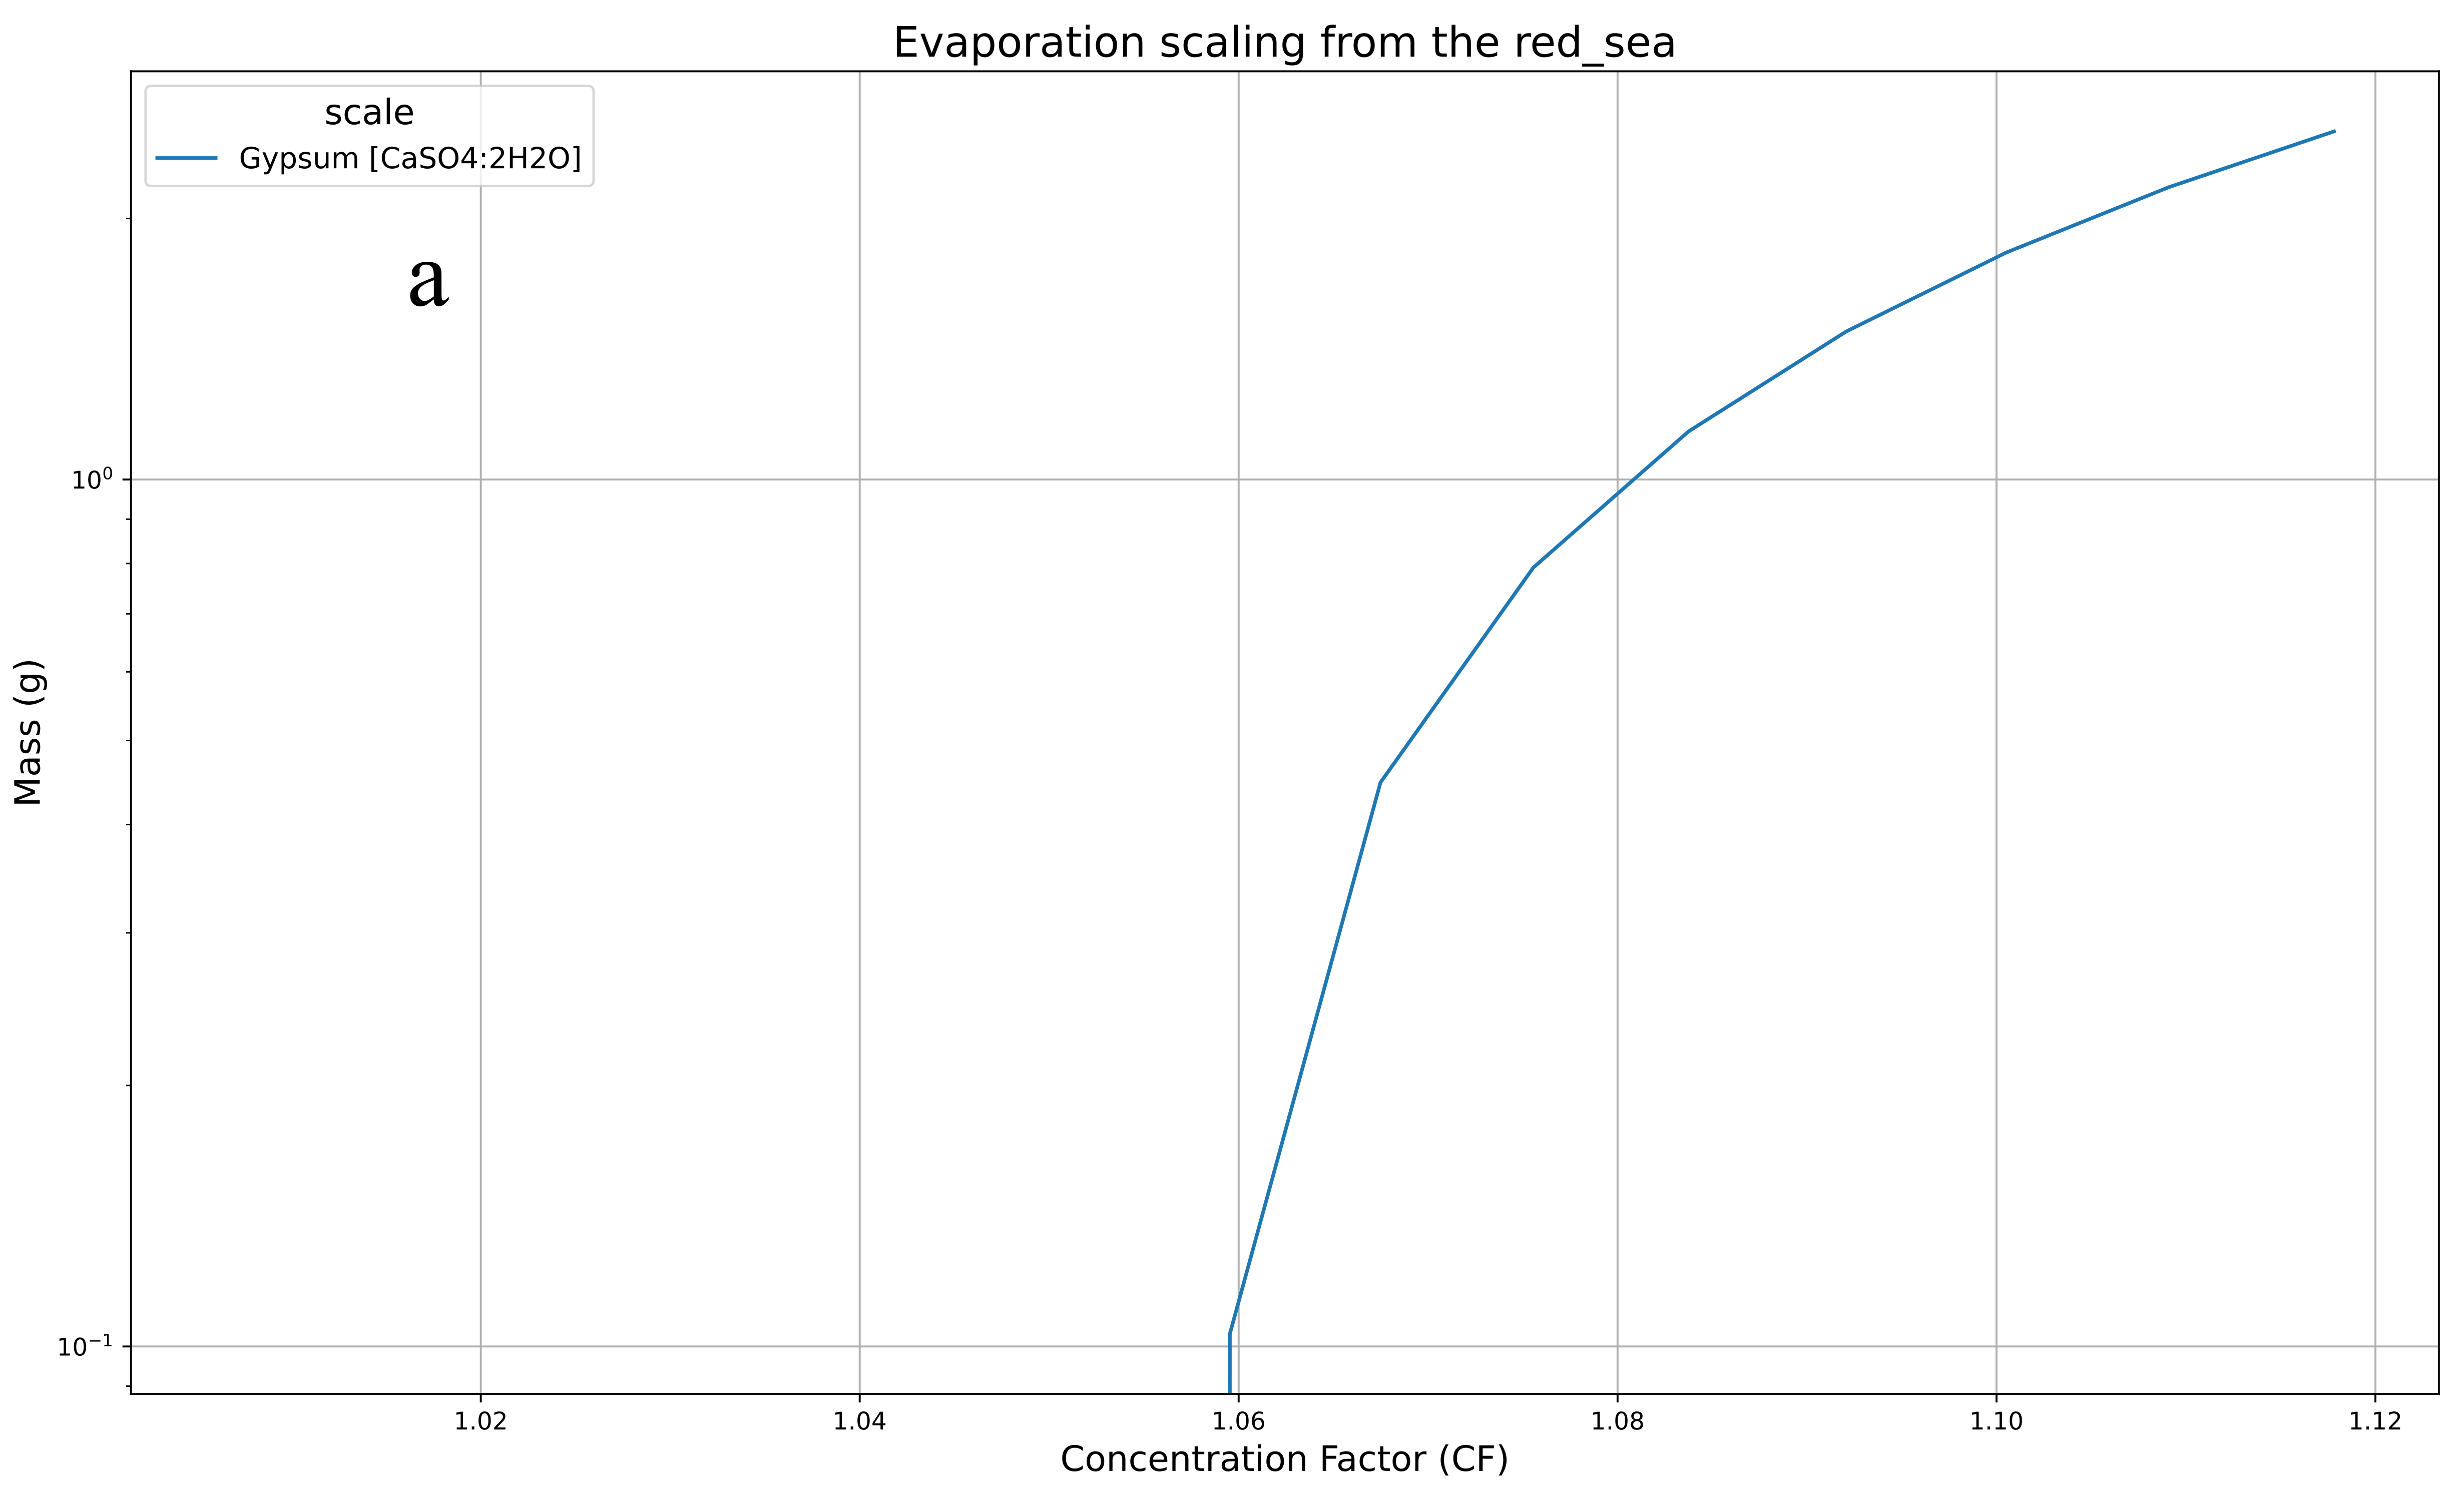
\includegraphics[width=\linewidth]{images/ROSSpy/sensitivity_analyses/evaporation/evaporation.png} \\ \midrule
    & 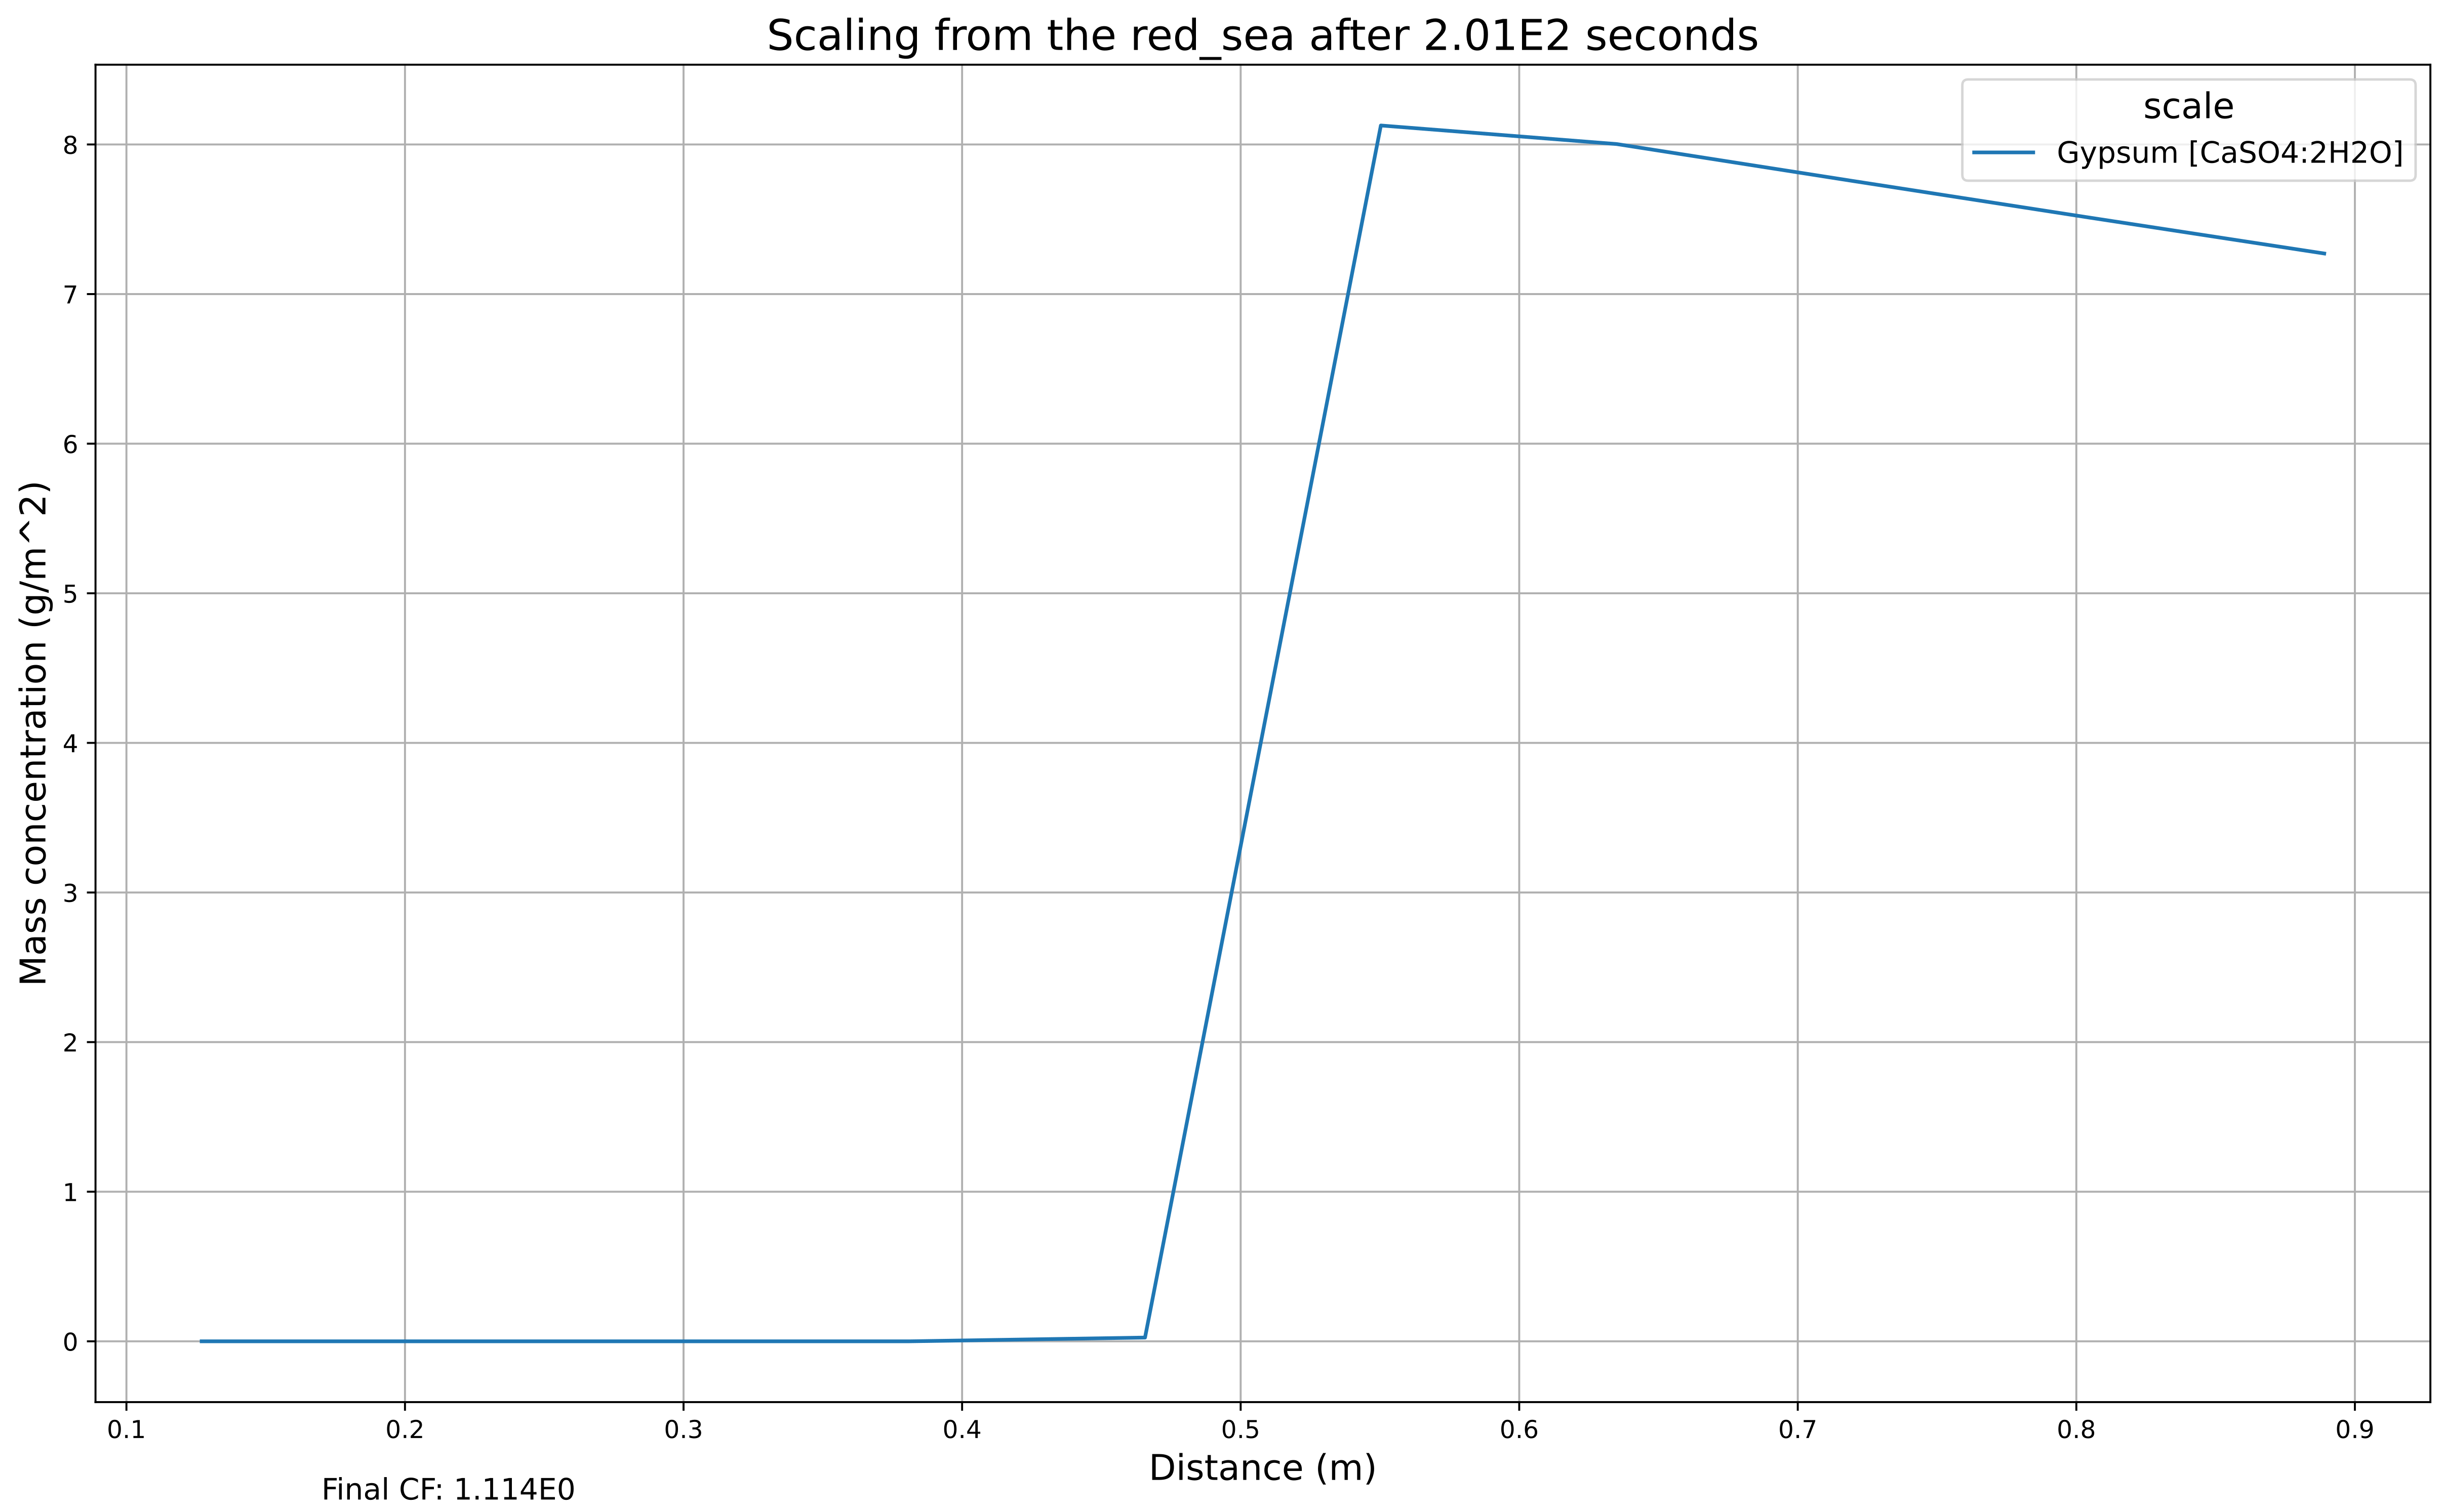
\includegraphics[width=\linewidth]{images/ROSSpy/sensitivity_analyses/evaporation/desalination.png}
    \caption{
        Scaling masses from Red Sea simulations of evaporation and desalination reactive transport. The scaling predictions between the two simulations are qualitatively identical. The final scaling mass from evaporation, however, is quantitatively less than that of desalination transport, even after accounting for the accumulation amongst different pore volumes: i.e.  3.36 grams versus 5.27 grams. This is attributed to the accumulation of scale over multiple timesteps within the same pore volume. 
    }
    \label{evaporation}
\end{figure}


\subsection{In-series RO arrangements}

In-series arrangements of multiple RO modules are represented by compounding individual modules. We determined that this approach is preferential to a few other methods: e.g. amplifying the characteristics of a single RO module in Table \ref{RO_dimensions} by a scalar $r$
\begin{equation}
    r=\frac{\Phi_{\Delta module,multi}}{\Phi_{\Delta module}},
\end{equation}
where the $\Delta \Phi_{multi-module}$ is the total permeate flux of the multi-module system, which can be either directly parameterized or approximated through eq. (8). The substitution of $CF_{multi}$ for $CF_e$ and $\Delta \Phi_{multi-module}$ for $\Phi_e$ into eq. (9) permits calculating $\Delta \Phi_{multi-module}$. 

\subsection{Water bodies}

Additional feed parameter files can be composed by emulating the organization of the default feed parameter files, and updating ionic concentrations and feed conditions. Literature sources that may provide these feed conditions for a range of potential feed water sources are provided in Table \ref{new_water_bodies}, although, the sources must be vetted to ensure that the studies measure the appropriate water depth and other factors of the desired feed. 

\begin{savenotes}
\begin{table}[!h]
    \centering
    \begin{tabular}{|c|c|c|}
        \toprule
        \textbf{Parameter} & \textbf{Value} & \textbf{Source} \\ \midrule
        
        \multicolumn{3}{c}{Module (meters)} \\ \midrule
        length & 1.016 & BW30-400 \cite{2020FilmTecElement} \\ 
        diameter & 0.201 & BW30-400 \cite{2020FilmTecElement}\\
        permeate tube diameter & 0.029 & BW30-400 \cite{2020FilmTecElement}\\ \midrule
        
        \multicolumn{3}{c}{Membrane (millimeters)} \\ \midrule
        filtration layer & 0.00025 & \cite{Pacheco2010CharacterizationTechniques,Jeong2007InterfacialMembranes} \\
        Feed spacer & 0.8636 & BW30-400 \cite{2020FilmTecElement} \& \cite{Sablani2002InfluenceSystems} \\
        Permeate spacer & 0.3 & \cite{} \\
        Polysulphonic layer & 0.05 & \cite{} \\
        Support layer & 0.15 & \cite{} \\
        Windings & 86 & BW30-400 
        \footnote{We calculated this quantity from the total thickness of the filtration section of the module, divided by the thickness of each individual membrane.}\\ \midrule
        
        \multicolumn{3}{c}{Membrane cross-section ($meters^2$)} \\ \midrule
        Module & 0.0317 & BW30-400 \cite{2020FilmTecElement}\\
        Permeate tube & 0.000661 & BW30-400 \cite{2020FilmTecElement}\\
        Filtration section & 0.0311 & BW30-400 \cite{2020FilmTecElement}\\
        Feed channel & 0.0157 & BW30-400 \cite{2020FilmTecElement}\\ \midrule
        
        \multicolumn{3}{c}{Feed channel capacity} \\ \midrule
        Volume ($meters^3$) & 0.0159 & BW30-400 \cite{2020FilmTecElement}\\
        Mass (kg) & 15.86 & BW30-400 \cite{2020FilmTecElement}\\ \midrule

        \multicolumn{3}{c}{Fluid flow ($\frac{meters^3}{second}$)} \\ \midrule
        Permeate & 0.000463 & BW30-400 \cite{2020FilmTecElement}\\
        Max Feed & 0.00442 & BW30-400 \cite{2020FilmTecElement}\\ \bottomrule
        
    \end{tabular}
    
    \caption{
        General dimensions of an RO module, with the corresponding citations. The DOW FILMTEC BW30-400 RO module is the default module, based upon precedence from other software \cite{Li2012OptimalDesalination}.
    }
    \label{RO_dimensions}
\end{table}
\end{savenotes}

\begin{table}[h!]
    \centering
    \begin{tabular}{|c|c|}
        \toprule
        \textbf{Water body} & \textbf{Geochemical measurements} \\
        \midrule
        Indian Ocean & \cite{Danielsson1980CadmiumWater,Nisha2014GeochemicalIndia,Stephen-Pichaimani2008EnrichmentIndia,Selvaraj2004EvaluationApproaches,Thangadurai2005Pre-tsunamiIndia,ParvezAl-Usmani2015TraceIndia,Sabine2002InorganicProcesses,Singh2013InternalBengal} \\
        Sargasso Sea & \cite{Bender1976DissolvedSea,Stoffyn-Egli1984MassOceans} \\
        South China Sea & \cite{Calvert1993GeochemistrySeas,Wen2006PhysicochemicalSea,Du2020DynamicsStudy,Chen2001NutrientBasin,Nakaguchi2004DissolvedSea} \\
        Greek Coast & \cite{Chester1981TheSediments,Voutsinou-Taliadouri1983DistributionGreece,Voutsinou-Taliadouri1997DissolvedSeawater} \\
        Toyko Bay & \cite{Fukushima1992TraceJapan} \\
        California Coast & \cite{Hershelman1981MetalsOutfall,Luoma1988DistributionBay,Biller2013SourcesSeason} \\
        North Atlantic & \cite{Loring1978GeochemistryLawrence.,Loring1979GeochemistryLawrence,Yeats1983PotentialAtlantic,Bothner1998MetalTime,Campbell1980BaselineBay,Gaulier2019TraceWaters,Statham1986Dissolved0-35N,Mohamed2011DissolvedOcean,Guay1998ASeas} \\
        Baltic Sea & \cite{Szefer1995DistributionSea,Kremling1978TheStation} \\
        North Pacific & \cite{Tanita2015SurfacePacific,Sim2019Annual20102013} \\
        South Pacific & \cite{Boyle1975CopperZealand,Boyle1976OnCadmium} \\
        General natural waters & \cite{Alibo1999RareOxidation,Klinkhammer1983RareVents,Garcia-Solsona2020RareSea,Longinelli1967Oxygen-18Lakes,Llyod1967Oxygen-18Sulfate,Culkin1966SodiumWater,Krumgalz1982CalciumWaters} \\
        Mississippi Salt Dome Basin & \cite{Kharaka1987GeochemistryU.S.A.} \\
        \bottomrule
    \end{tabular}
    \caption{
        Proposed literature of potential feed water that can constitute new parameter files.
    }
    \label{new_water_bodies}
\end{table}

\subsection{Dual domain}

\begin{figure}[h!]
    \centering
    \begin{tabular}{c|c}
        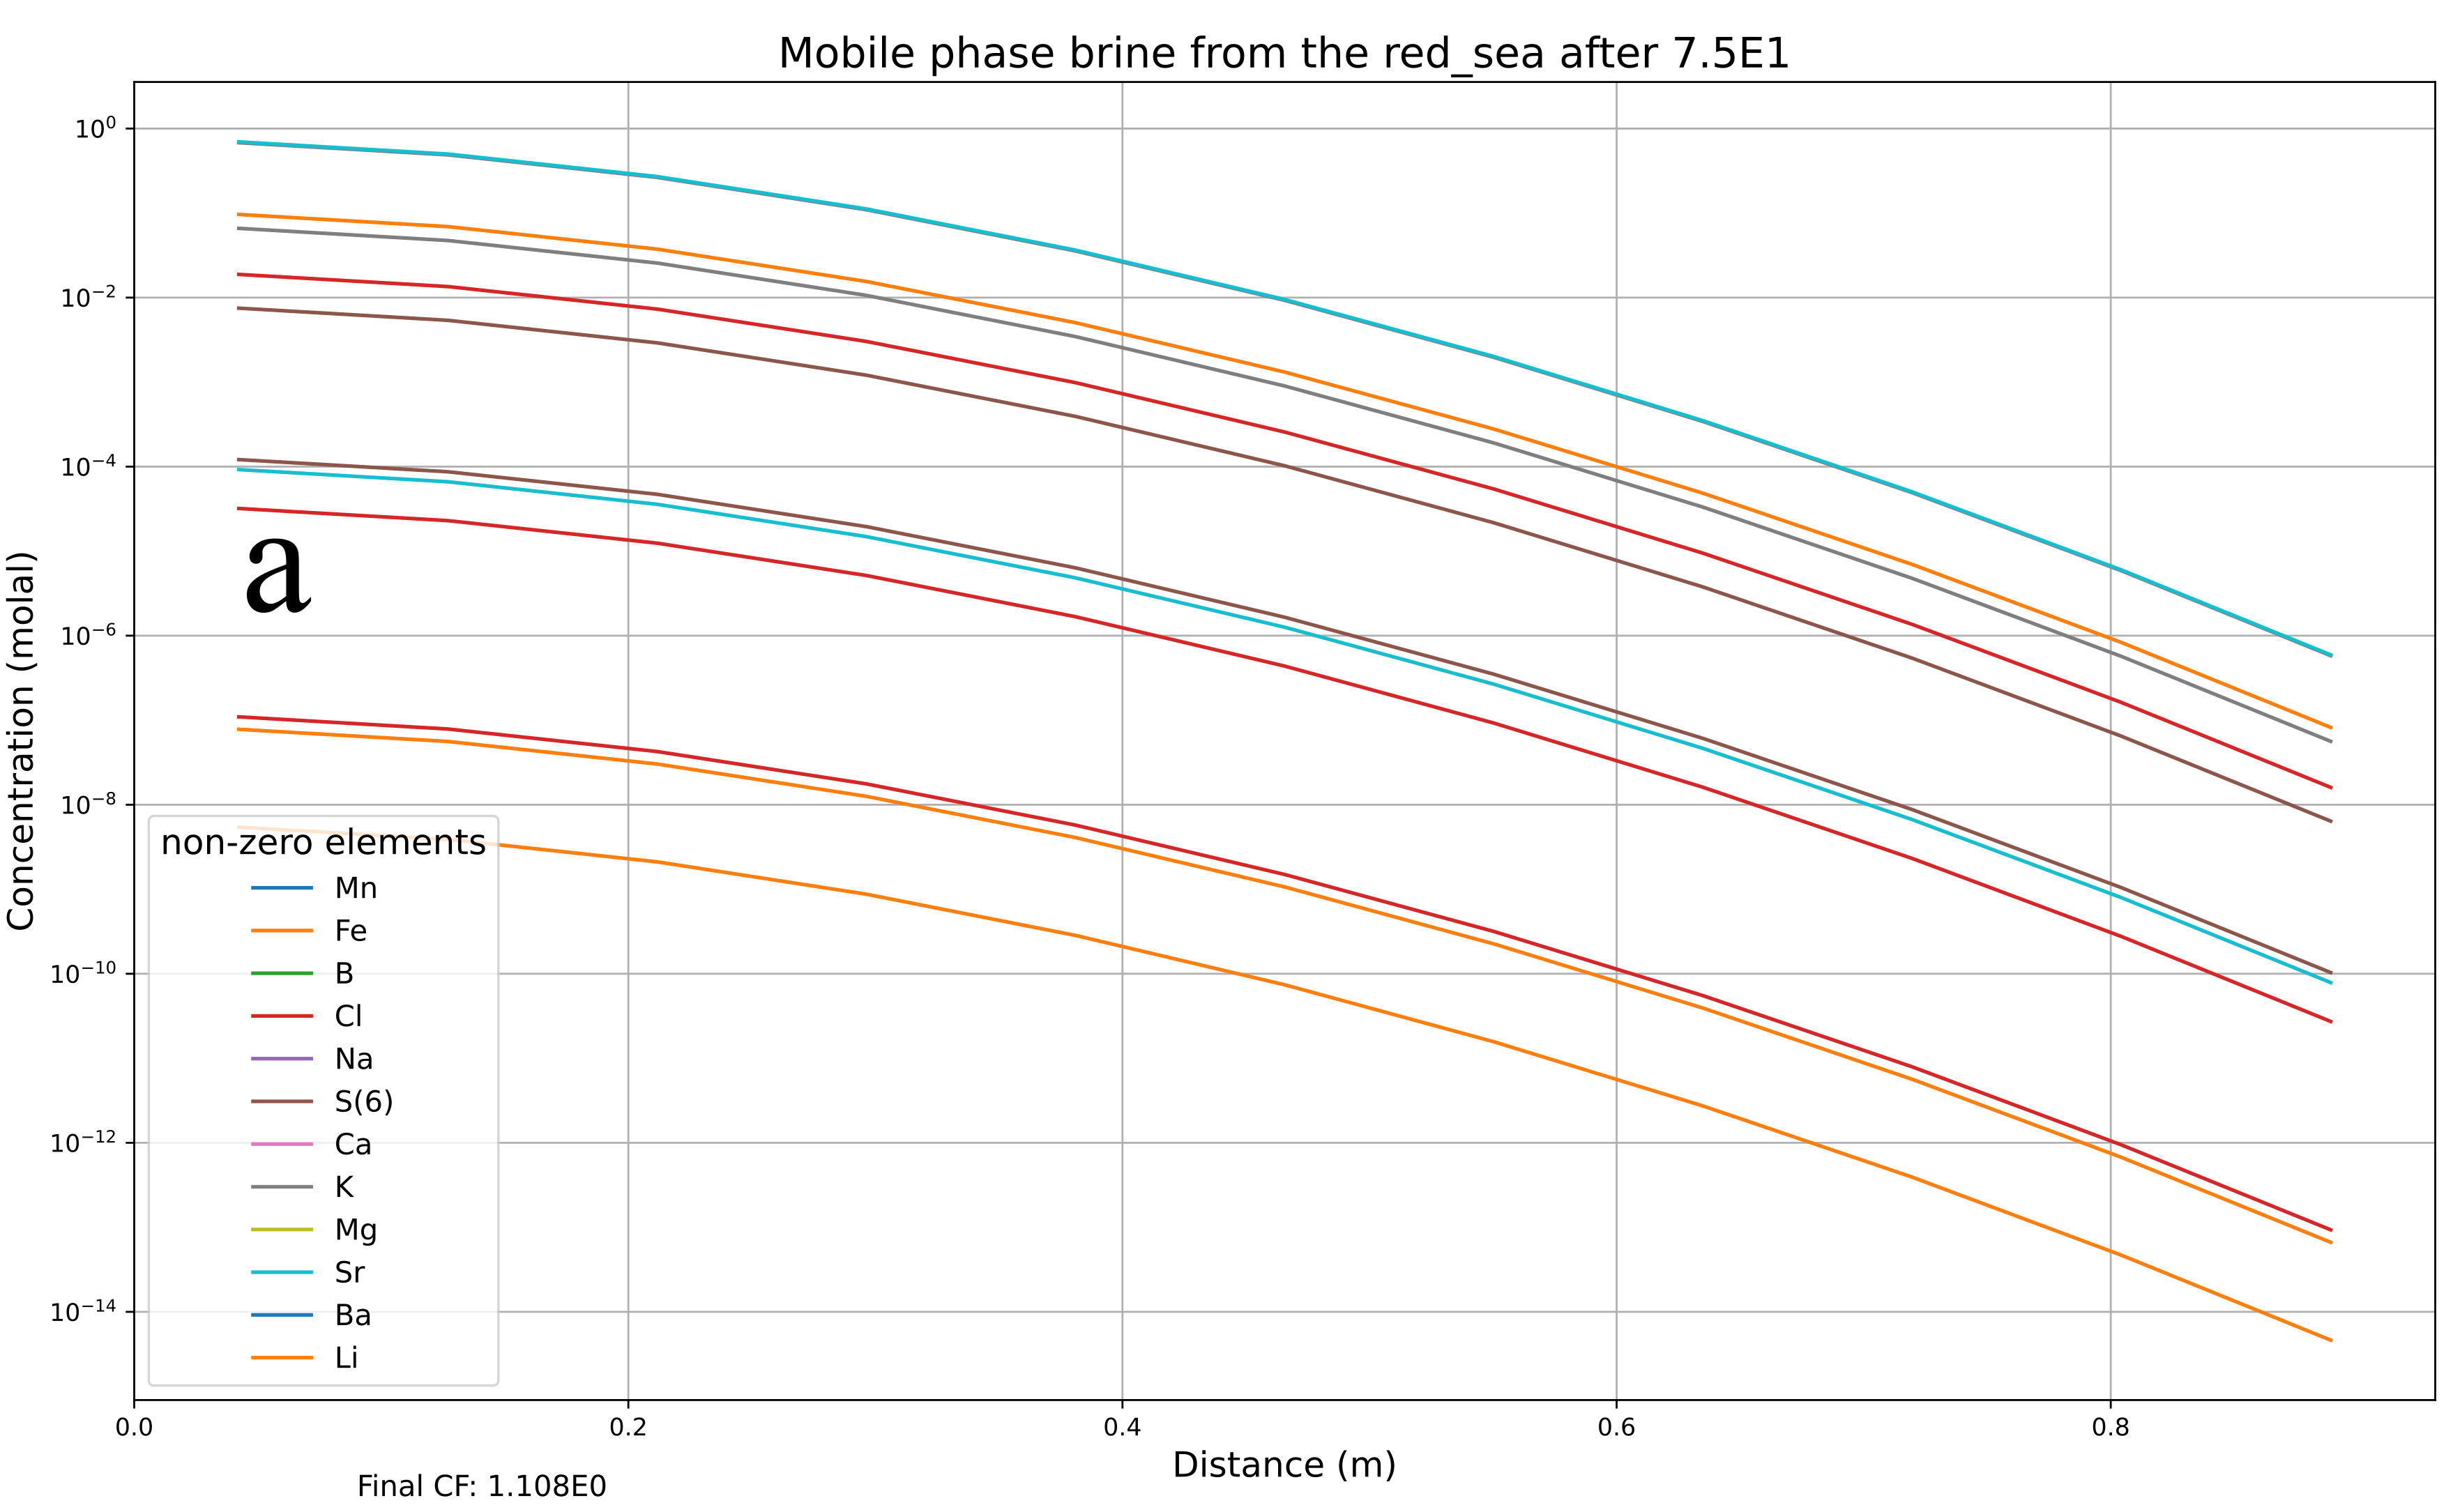
\includegraphics[width=0.49\textwidth]{images/ROSSpy/sensitivity_analyses/EF/mobile_large_ef.png} &
        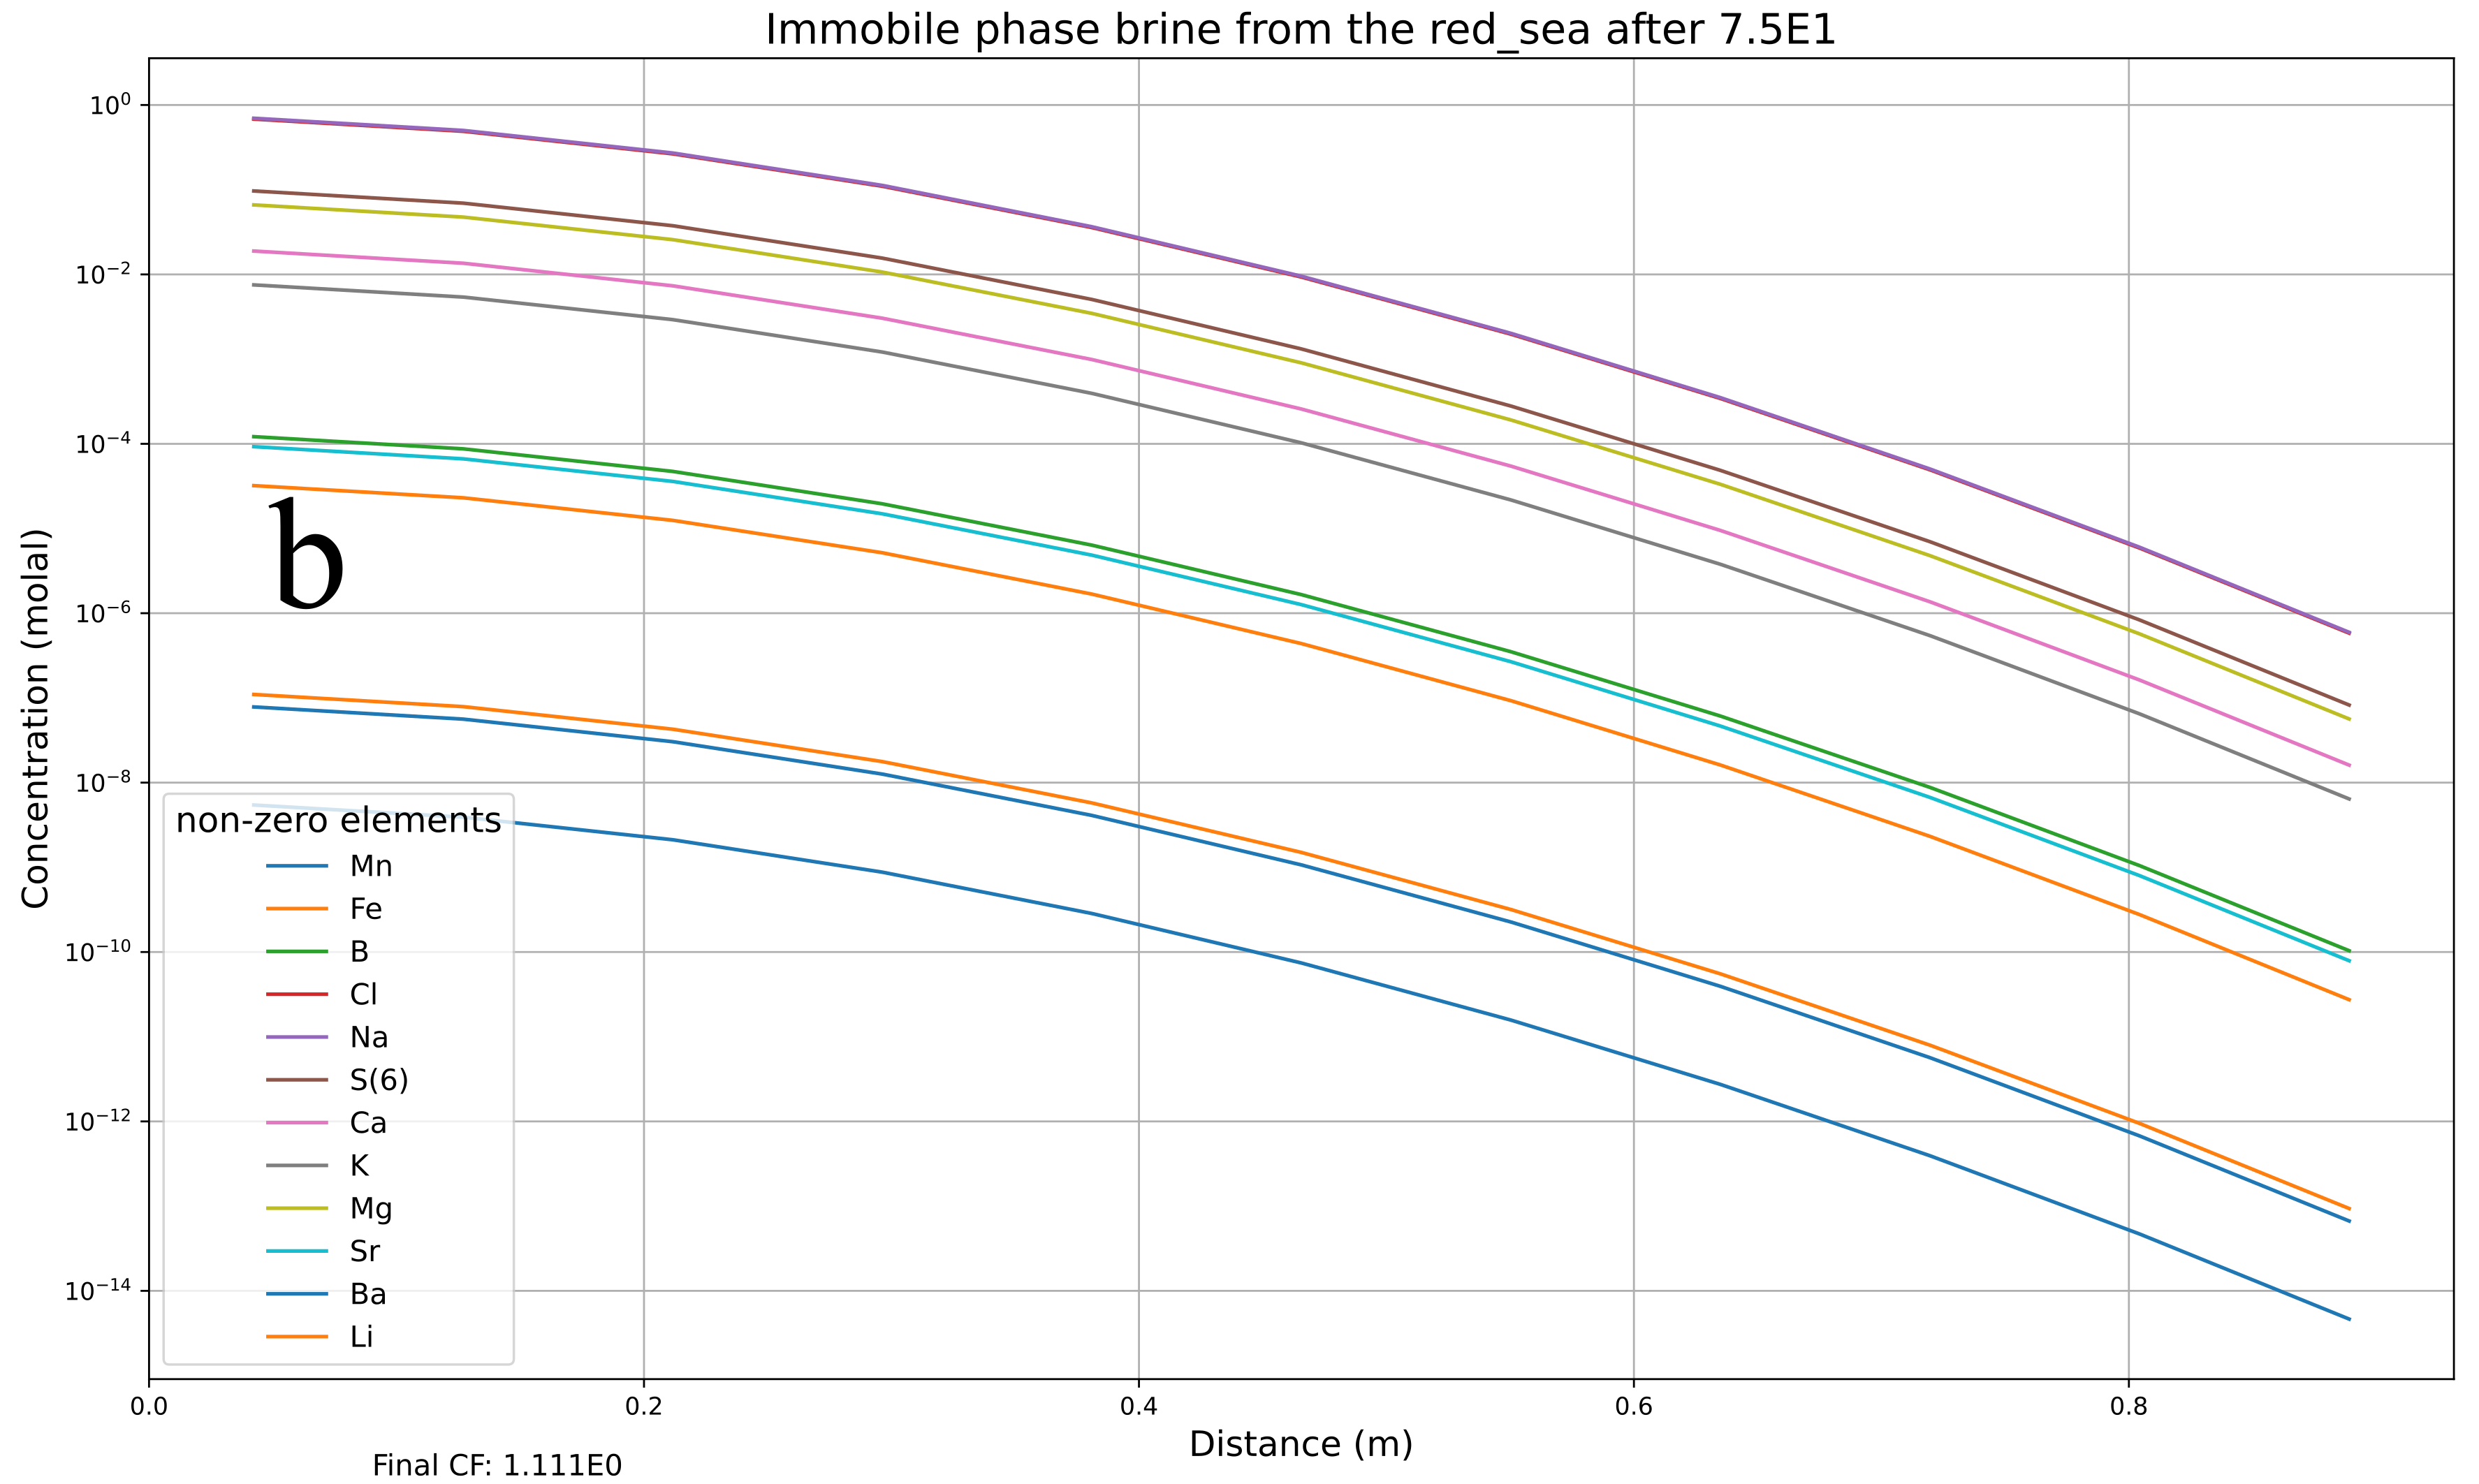
\includegraphics[width=0.49\textwidth]{images/ROSSpy/sensitivity_analyses/EF/immobile_large_ef.png} \\ \midrule
        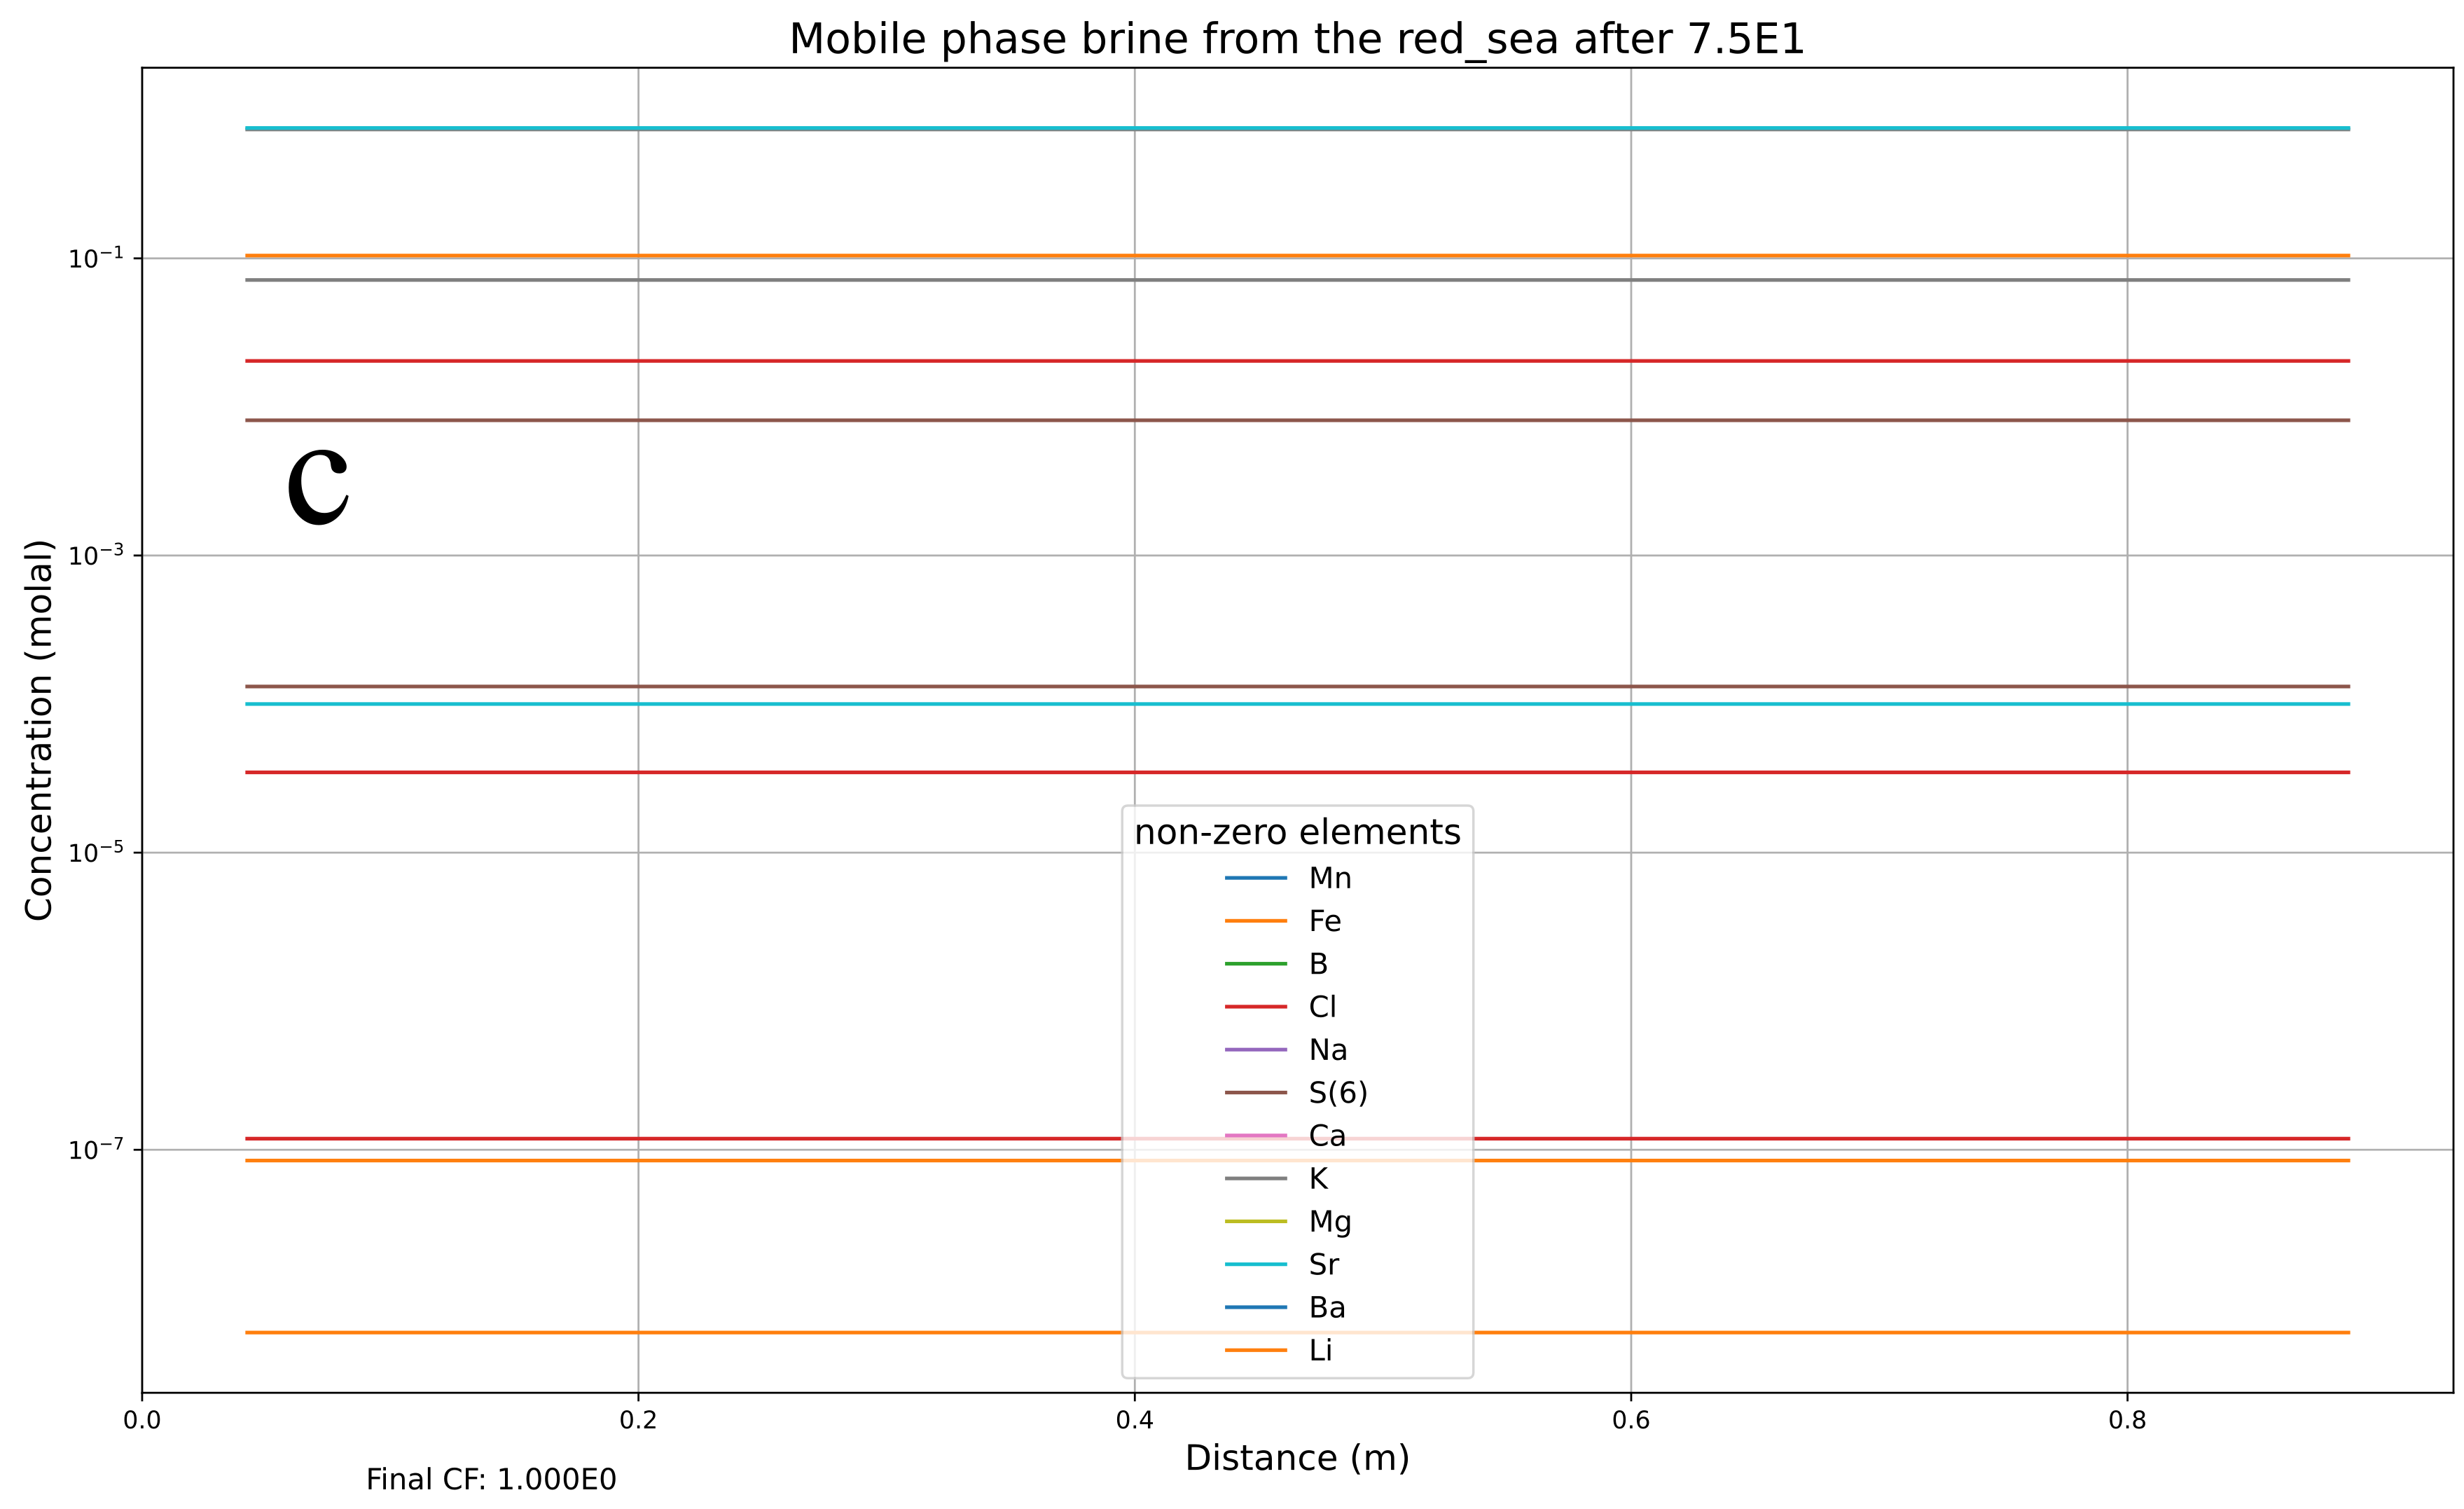
\includegraphics[width=0.49\textwidth]{images/ROSSpy/sensitivity_analyses/EF/mobile_small_ef.png} & 
        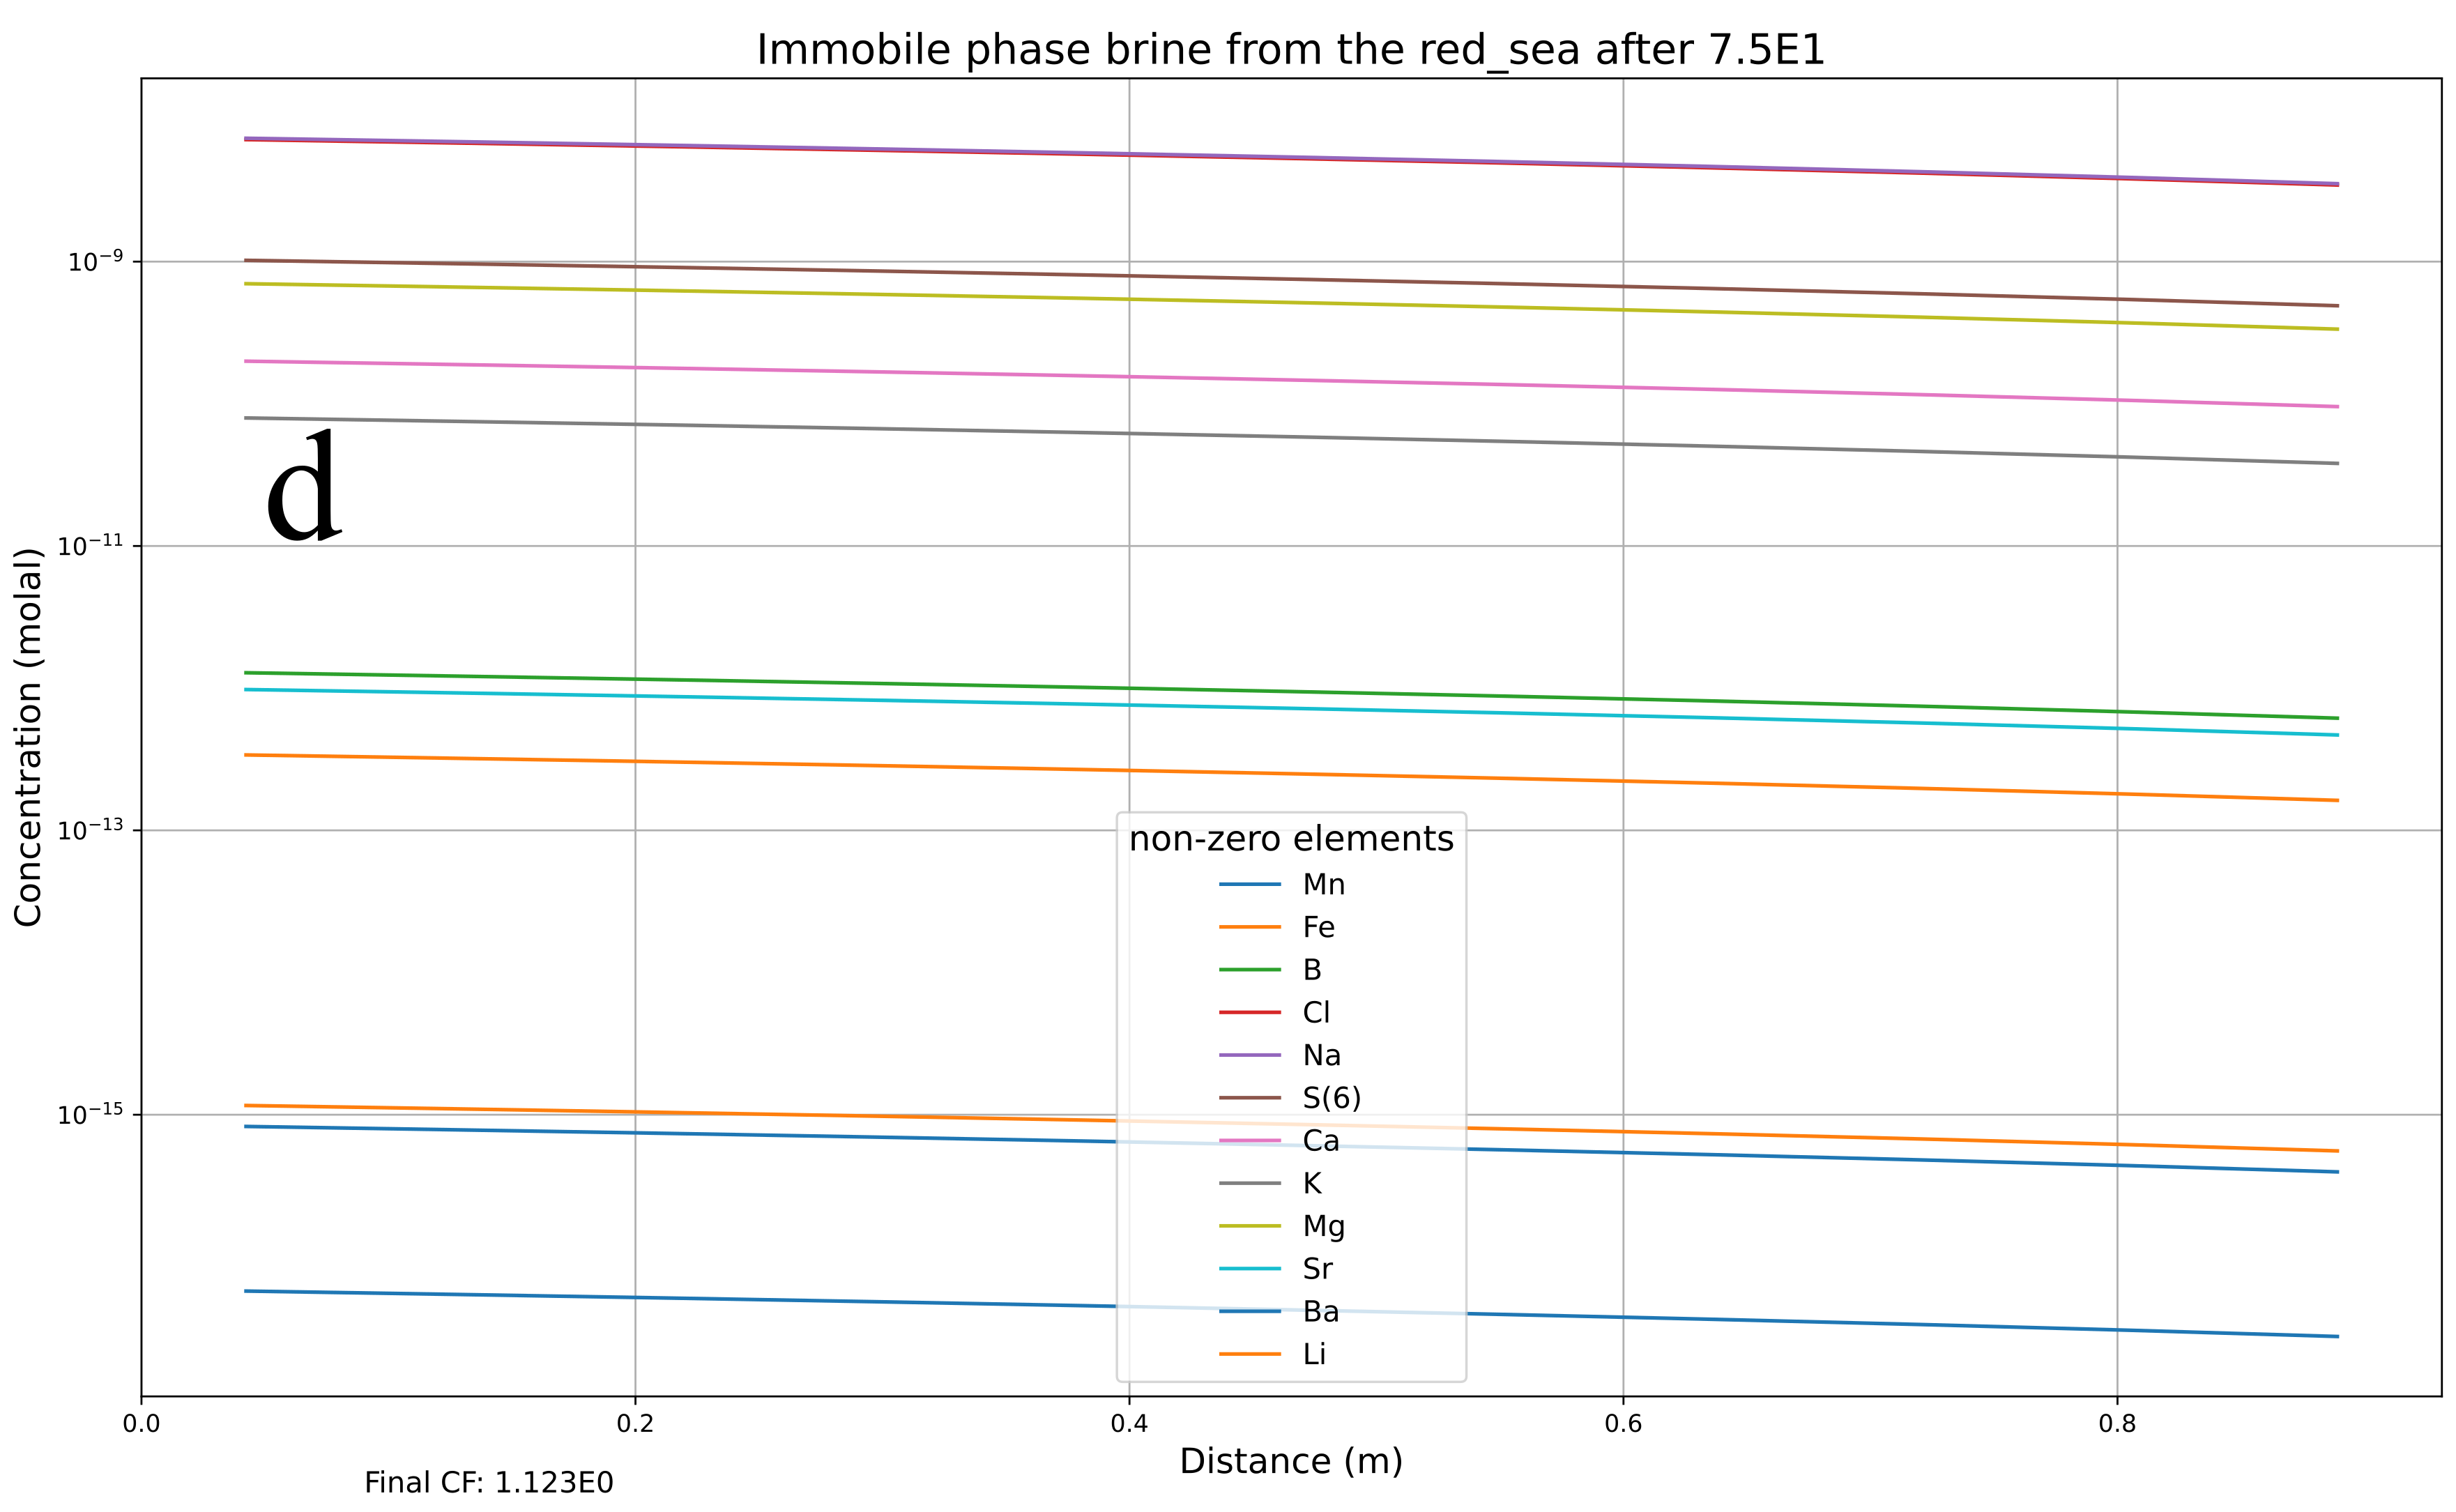
\includegraphics[width=0.49\textwidth]{images/ROSSpy/sensitivity_analyses/EF/immobile_small_ef.png} \\ \bottomrulerule
    \end{tabular}
    \caption{
        Scaling predictions from different exchange factor (EF) parameter values of the otherwise same simulation, which are the $\frac{1}{sec}$ rate constant of solvent exchange between the mobile and immobile phases. Panels a) and b) depict the mobile (bulk) and immobile (CP) phases of a simulation with $EF=1E10$, while panels c) and d) depict the mobile and immobile phases of a simulation with $EF=1E-10$, respectively.
    }
    \label{ef_values}
\end{figure}

ROSSpy represents the feed solution environment as a single domain, despite that the dual-domain model is more fundamentally accurate. Our original approach of representing the dual-domain model in PHREEQ code, which is the bottleneck for using this solution model, is through representing the mobile phase (bulk) as  one set of cells -- $[1,n]~n\in W$ -- and representing the immobile phase (CP) as a second set of cells -- $[n+2,m]~m \in W>n+2$. These sets of cells exchange solvent with a parameterized rate, which in PHREEQ code is termed the Exchange Factor (EF). Our investigations of this approach have revealed peculiar phenomena in Figure \ref{ef_values}, where the brine appears to be diluting -- instead of concentrating -- over the module distance, independent of the EF exchange parameter value. Scaling phenomena, which are detailed in the dual-domain example Notebook of our GitHub, are also not sensible. We are continuing to explore PHREEQ code for a method of implementing dual-domain reactive transport, and we encourage any users or researchers to share ideas toward this end.

\subsection{PHREEQ}
PHREEQ code is the geochemical basis of ROSSpy. The PHREEQC manual details most of these calculations, and the most pertinent calculations to ROSSpy are summarized in the following section.

\subsubsection{PHREEQ calculations}
The total concentration $\Psi_i$ of ionic species $i$ is calculated in each timestep, 
\begin{equation} \label{total_species_concentration}
    \Psi_i=C_i+\sum_{i=1}^{N_x}(v_{ij}*C_j),
\end{equation}
where $C_i$ is the molal concentration of dissolved $i$; $N_x$ is the linearly dependent set of chemical reactions that involve $i$; $C_j$ is the molal concentration of compound $j$ that contains $i$; and $v_{ij}$ is the stoichiometric coefficient for the moles of $i$ per mole of compound $j$. The mineral dissolution-precipitation equilibria over the simulation time $t$ is calculated through a similar equation, 
\begin{equation} \label{concentration_change}
    \frac{\partial \Psi_i}{\partial t}=\sum_{m=1}^{N_m}(\nu_{mj}*R_m),
\end{equation}
where $N_m$ is the set of reactions that include specie $i$; $v_{mi}$ is the stoichiometric coefficient for the moles of $i$ per mole of mineral $m$; and $R_m$ is the reaction flux of dissolution or precipitation for $(+)$ and $(-)$, respectively,
\begin{equation} \label{mineral_precipitation_reaction}
    R_m=sgn[\Omega]*A_m*k_m*(\Pi(a^n)) |e^{\frac{\eta*\Delta G}{RT}}-1|^p,
\end{equation}
where $\Omega=log⁡\frac{Q_{dissolution}}{K_{sp}} and, for the simulated mineral $m$, $A_m$ is the reacting surface area; $k_m$ is the rate constant of dissolution or precipitation; $Q_m$ is the ion activity product constant; and $\eta$ and $p$ are experimentally determined parameters. The $|e^{\frac{\eta * \Delta G}{RT}}-1|^p$ term of \cref{mineral_precipitation_reaction} simplifies to $1$ for irreversible precipitation or dissolution. The set of \cref{total_species_concentration,concentration_change} necessitates that any perturbations to ionic concentrations $\frac{\partial \Psi_i}{\partial t}$ manifest from complexation equilibria. The molal concentration $C_j$ of compound $j$ is discerned,
\begin{equation}
    C_j=\frac{\Pi_{j=1}^{N_c} (\gamma_j*K_j )^{v_{ij}}}{\gamma_j*K_j},
\end{equation}
where $N_c$ is the set of linearly independent chemical reactions; $\gamma_j$ is the activity coefficient of compound $j$; and $K_j$ is the equilibrium constant
\begin{equation}
    K_j=a_j \Pi_m^{M_{aq}} (a_m)^{-v_{m,j}},
\end{equation}
where $M_{aq}$ is the number of minerals in the aqueous system; $v_{m,i}$ is the stoichiometric coefficient of compound $j$ per mole of mineral $m$; and $a_j$ and $a_m$ are the activity coefficients of compound $j$ and mineral, respectively. The activity coefficient $\gamma_j$ is calculated through either the Debye-Hückel model \cite{Aqion2016ActivityModels},
\begin{equation}
    log⁡(\gamma_j)=-A*z_j^2\sqrt{\mu},
\end{equation}
the WATEQ Debye-Hückel model \cite{Aqion2016ActivityModels},
\begin{equation}
    log⁡(\gamma_j)=\frac{-A*z_j^2*\sqrt{\mu}}{1+B*a_j^0*\sqrt{\mu}}+b_j \mu,
\end{equation}
the Davies model \cite{Davies1938TheSulphates},
\begin{equation}
    log⁡(\gamma_j)=-A*z_j^2 (\frac{\sqrt{\mu}}{1+\sqrt{\mu}}-0.\mμ),
\end{equation}
or the empirical Pitzer model \cite{Pitzer1973ThermodynamicsEquations}, where $A$ and $B$ are experimentally determined parameters; $a_j^0$ and $b_j$ are fitted parameters; $z_j$ is the charge of compound $j$; and $\mu$ is the ionic strength of the solution. The ionic strength is separately calculated
\begin{equation}
    \mu=\frac{1}{2}\sum_{j=1}^{N_{aq}}z_j^2 \frac{n_j}{W_{aq}},
\end{equation}
where $W_{aq}$ is the simulated water mass and $n_j$ 
\begin{equation}
    n_j=C_j*W_{aq}=\frac{K_i*W_{aq}}{\gamma_j*(\Pi_m^{M_{aq}} (a_m)^{v_{m,j}}}
\end{equation}
is the moles of compound $j$. These calculations and geochemical models are more thoroughly described in the PHREEQC manual and in peer-reviewed literature on the subjects.

% \bibliography{mendeley_references.bib}